%!TEX root = ../../diachron-D5_2.tex

\subsection{High-Level Architecture}
\label{sec:HLA} 

The purpose of the Quality Framework is to provide an integrated platform that: 
\begin{enumerate}
\item assesses RDF datasets and triple stores in a scalable manner;
\item provides queryable quality metadata on the assessed datasets;
\item provides visualisations on the quality 
\end{enumerate}
Furthuremore, we aim to create an infrastructure and a platform that (i) can be easily extensible by different third party by creating their custom and more specific pluggable metrics required to assess their particular dataset domain, and (ii) having the the necessary ontology framework to represent the metadata about the quality of the assessed linked datasets.

Currently, there is no uniform infrastructure to address the quality assessment problem, allowing the extension or redefinition of custom-specific metrics such as those required by the DIACHRON use cases.
Tools such as Trellis~\cite{Gil2002}, WIQA~\cite{Bizer2008:PhDThesis:biblatex} and Sieve~\cite{Mendes2012} implement a number of metrics but lacked flexibility wrt the level of automation, and user friendliness~\cite{Zaveri2013}. 

\begin{figure*}[tbph]
\center
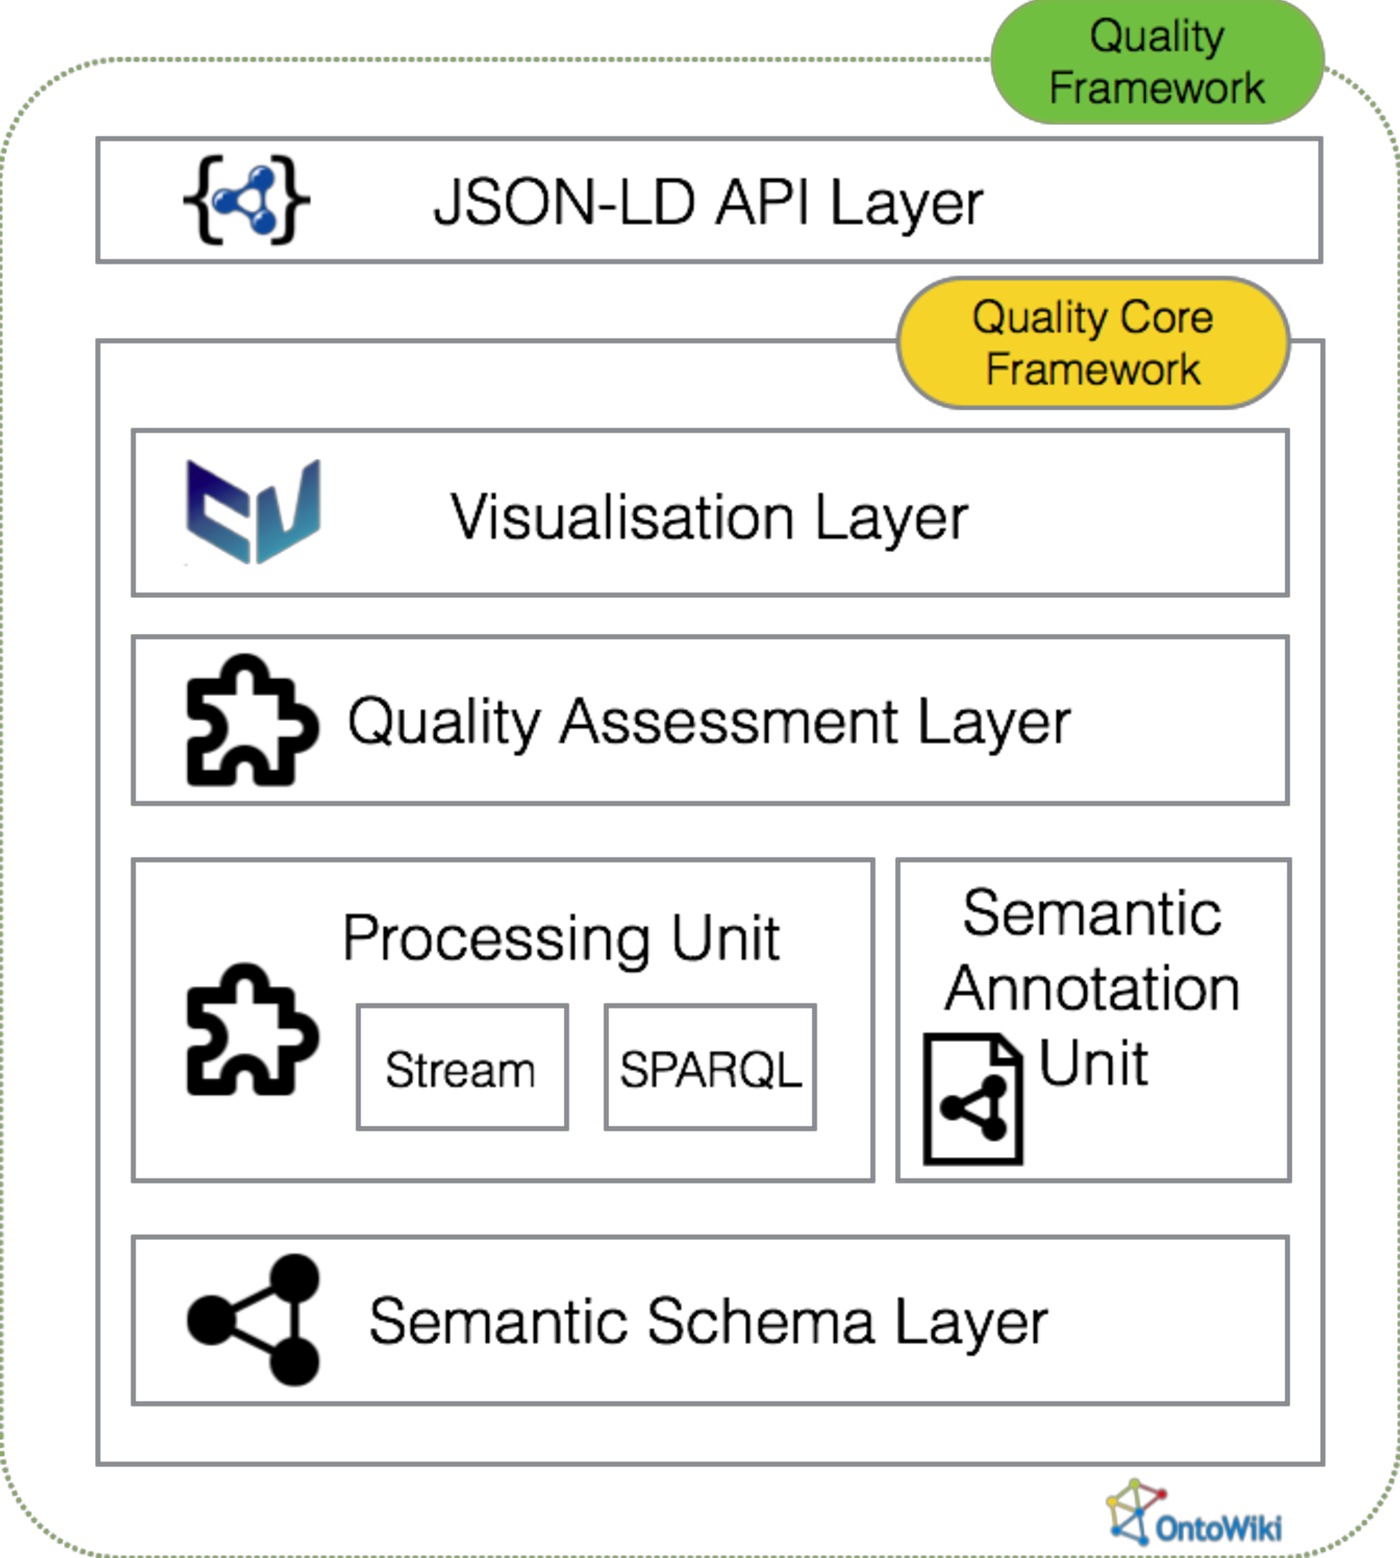
\includegraphics[scale=0.3]{images/qualityFrameworkHLA.pdf} 
\caption{Quality Framework High Level Architecture Design} 
\label{fig:qualityFramework}
\end{figure*}

Figure~\ref{fig:qualityFramework} illustrates the high level architecture of the Quality Framework.
The two main components are the API layer (cf. Section~\ref{sec:RestAPI}) and the Core framework.
The core framework is made up of five modules: \emph{Semantic Schema Layer}, \emph{Processing Unit}, \emph{Semantic Annotation Unit}, \emph{Quality Assessment Layer}, and \emph{Visualisation Layer}.

\subsubsection{Semantic Schema Layer}
The Quality Framework is based on semantic technologies and thus has an underlying semantic vocabulary layer which currently is made up of two ontologies: (i) the Dataset Quality Ontology (daQ)\footnote{\url{http://purl.org/eis/vocab/daq}}; and (ii) the Quality Problem Report Ontology (qr)\footnote{\url{http://purl.org/eis/vocab/qr}}. 
The former describes the quality metadata representation whilst the latter describes quality problems found in the dataset itself. 
The semantic schema layer is meant to be domain independent, where it could be reused in other similar frameworks. 
The daQ ontology (cf. Section~\ref{sec:DAQ}) is the core vocabulary of this schema layer, and any other ontology part of this layer builds upon it.

The daQ ontology is a comprehensive generic vocabulary framework, based on three abstract concepts (Category, Dimension and Metric). 
Any newly implemented specific metric should have its representation in RDF, extending the daQ ontology. In DIACHRON, all metrics are defined in the Diachron Quality Metric vocabulary (dqm)\footnote{\url{http://purl.org/eis/vocab/dqm}}. 
Such vocabularies are easily integrated in the Quality Framework, since they adopt and extend the generic daQ vocabulary (by inheriting class and properties) as the way quality metadata is represented (cf. Section~\ref{sec:extendingDAQ}).
The Quality Problem Report Ontology (qr) is made up of two classes a \texttt{qr:QualityReport} and \texttt{qr:QualityProblem}. 
The former represents a report on the problems detected during the assessment of quality on a dataset, whilst the latter represents a quality problem detected during the assessment of quality metrics on triples. 
Four properties are also defined in the ontology. 
The \texttt{qr:computedOn} represents the dataset URI on quality assessment has been made. 
This property is attached to a \texttt{qr:QualityReport}. \texttt{qr:hasProblem} links a \texttt{qr:QualityProblem} to a \texttt{qr:QualityReport}. 
The mentioned property identifies problem instances in a report. 
Each \texttt{qr:QualityProblem} \texttt{isDescribedBy} an instance of a \texttt{daq:Metric}\footnote{refer to Section~\ref{sec:DAQ}}. 
The property \texttt{qr:problematicThing} represent the actual problematic instance from the dataset. This could be a list of resources (\texttt{rdf:Seq}) or a list of reified statements.
Listing~\ref{lst:dataset_qr} represents an excerpt from a typical dataset showing the instance of \texttt{ex:JoeDoe} who is a \texttt{foaf:Researchers} working for \texttt{ex:UniBonn}.
In these two instances there are three problematic triples:
\begin{description}
\item [(A) $\langle$ \texttt{ex:JoeDoe a foaf:Researcher} $\rangle$] - The problem in this triple is caused by the usage of an undefined class, in this case \texttt{foaf:Researcher};
\item [(B) $\langle$ \texttt{ex:JoeDoe rdfs:label "JoeDoe"} $\rangle$] - The literal ("JoeDoe") in the triple causes the malformed capitalisation metric to point out a problem in this triple;
\item [(C) $\langle$ \texttt{ex:UniBonn rdfs:label "UniBonn"} $\rangle$] - The literal ("UniBonn") in the triple causes the malformed capitalisation metric to point out a problem in this triple.
\end{description}
Listing~\ref{lst:qualityreport} represent these three problems using the Quality Problem Report ontology.
\lstinputlisting[caption={An excerpt of a typical Dataset},label=lst:dataset_qr, language=N3]{listings/qrtest.trig}
\lstinputlisting[caption={An corresponding Quality Report for Listing~\ref{lst:dataset_qr}},label=lst:qualityreport, language=N3]{listings/qualityreport.trig}

\subsubsection{Processing Unit}
The Processing Unit is an integral part of the Quality Framework.
In this framework, we provide two main scalable processing units: a sequential stream processor (cf. Section~\ref{sec:StreamProcessor}) and SPARQL processor\footnote{This processor is still being investigated and will not be ready by the deliverable deadline.}.
The former streams triples from RDF date dumps one by one in a sequential fashion.
The latter allows the framework to assess quality on data that is available only in SPARQL endpoints. 
This unit is one of the two extensible modules (the other being Quality Assessment Layer) in the Quality Framework.
For DIACHRON, the plan is to extend the sequential stream processor, enabling the de-reification of RDF statements into RDF triples.

Typically, an initialised processor has 2 inputs: the dataset URI (for the sequential stream processor) or the dataset SPARQL endpoint (in the case of the SPARQL processor), and a metric configuration file.
Listing~\ref{lst:conf_metric} shows an example of a typical metric configuration file.
\lstinputlisting[caption={An typical metric configuration file},label=lst:conf_metric, language=N3]{listings/conf.trig} 
Each data processor in the Quality Framework has a defined 3-stage procedure (Listing~\ref{lst:int_ioprocessor}): (i) processor initialisation; (ii) processing; and (iii) memory clean up.
In the first process (processor initialisation), the processor create the necessary objects in memory to process data and load the required metrics that are instructed in the configuration file.
Once the initialisation is ready, then processing is done by passing the streamed triples into the metrics.
Finally, memory clean up ensures that no unused objects are using unnecessary computational power.
\lstinputlisting[caption={IO Processor Interface},label=lst:int_ioprocessor, language=Java]{listings/ioprocessor.java} 

\subsubsection{Quality Assessment Layer}
The Quality Assessment Layer is unarguably the most important layer in this Quality Framework.
The framework can be extended by any third party providing their own custom specific metric.
This is already done in the DIACHRON project, where a number of metrics (cf. Section~\ref{sec:DQMetrics}) required to assess the various use cases specified in Deliverable ??? are implemented.
The Quality Assessment Layer provides two interfaces and an abstract class (cf. Figure~\ref{fig:classDiagram}) which facilitate the quality framework to be a pluggable and extensible platform.
The interface \texttt{QualityMetric} is the core interface class which describes the metric classes.
Each metric implementing this interface, must implement the following classes:
\begin{description}
\item[compute - ] This method assess the quad/triple which is passed by the stream processor by the defined metric;
\item[metricValue - ] This method returns the value computed by the quality metric;
\item[toDAQTriples - ] This method will return a list of daQ triples, containing quality metadata about the assessed metric, which will be stored in the dataset as a new named graph (quality graph);
\item[getMetricURI - ] This method returns the URI of the Quality Metric from the ontology description (e.g. \url{http://purl.org/eis/vocab/dqm#DereferenceablityMetric});
\item[getQualityProblems - ] This method returns a typed (List$\langle$Resource$\rangle$ or List$\langle$Quad$\rangle$) ProblemList which will be used to create a quality report of the metric;
\end{description}

\begin{figure*}[tbph]
\center
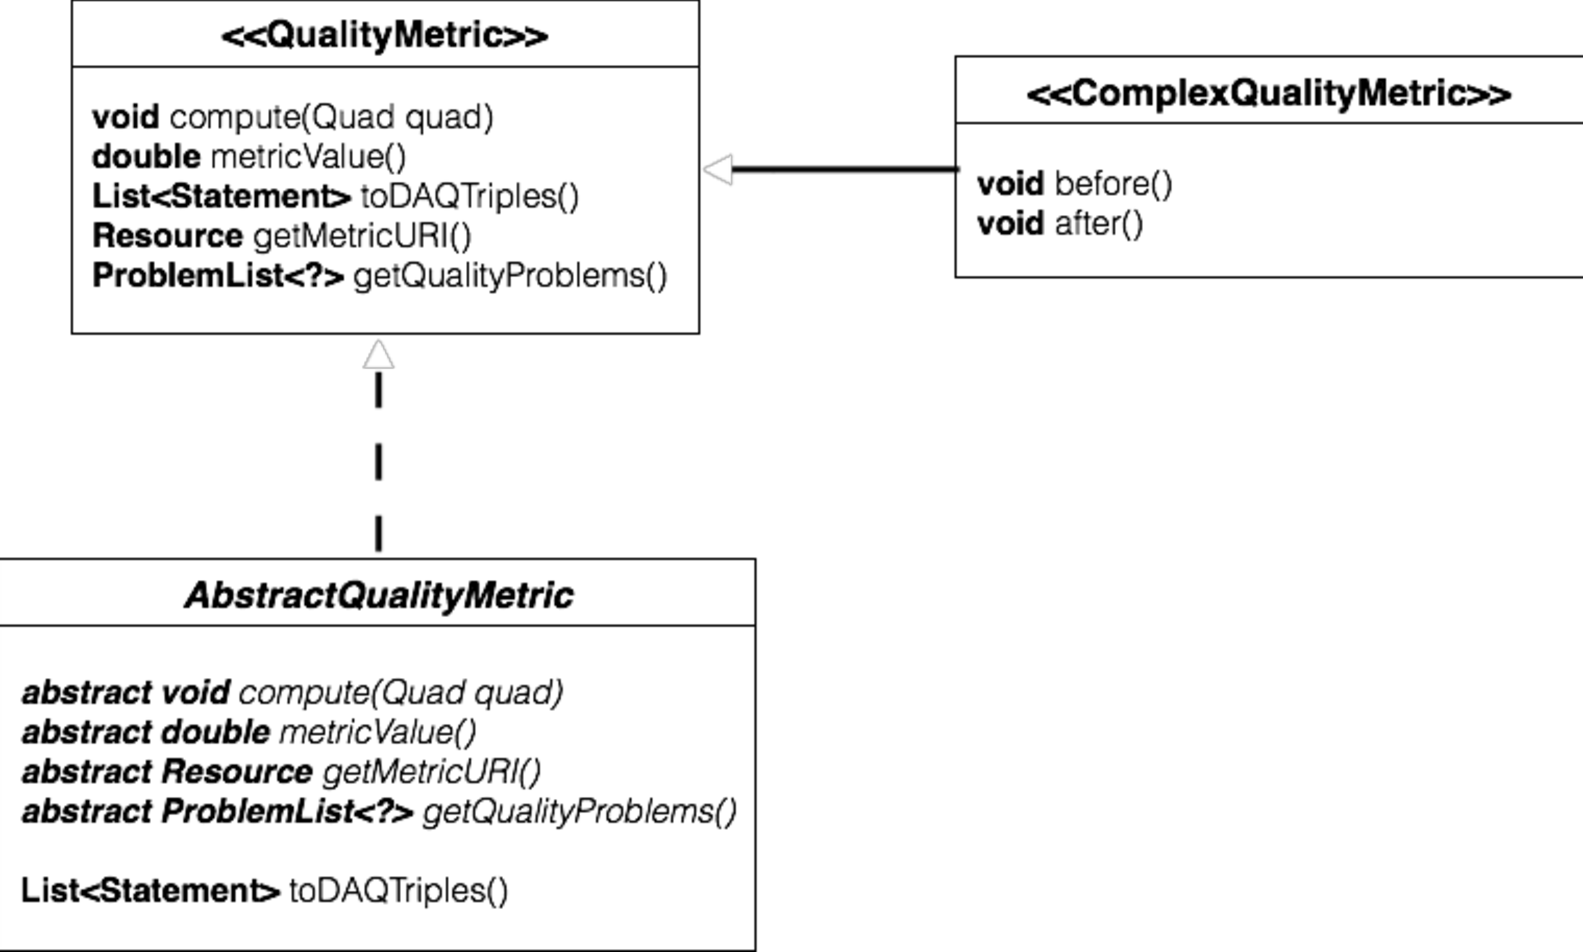
\includegraphics[scale=0.3]{images/classdiagram.pdf} 
\caption{Quality Assessment Layer Class Diagram - A Quality Framework as a Pluggable Platform} 
\label{fig:classDiagram}
\end{figure*}

Furthermore, a metric might require some pre-processing or post-processing.
Therefore, an interface (\texttt{ComplexQualityMetric}) extending \texttt{QualityMetric} was developed.
This interface allow metric developers to perform such processing using the \texttt{\textbf{void} before()} and \texttt{\textbf{void} after()} methods.

In order to facilitate further such development of pluggable metrics, the \texttt{AbstractQualityMetric} class was developed, implementing the \texttt{QualityMetric} interface.
In this abstract class, the method \texttt{List$\langle$Statement$\rangle$ toDAQTriples()} is implemented, generating daQ observation instances (cf. Section~\ref{sec:DAQ}) for the metric being assessed. 

\subsubsection{Semantic Annotation Unit}
The Semantic Annotation Unit takes the generated triples (from the \texttt{toDAQTriples()} method) in order to create the quality metadata in a dataset.
The unit provides a number of helper classes that provide inferencing queries on vocabularies that describe metrics (such as DQM) based on the core ontology daQ.
Therefore, RDF descriptions of metrics extending the daQ (cf. Section~\ref{sec:extendingDAQ}) ontology is absolutely required.
These inferencing queries enable the framework to create a complete metadata description (cf. Section~\ref{sec:DAQ}) of an assessed quality metric.

\subsubsection{Visualisation Layer}
\label{sec:vislayer_hla}
CubeViz is an OntoWiki\footnote{http://ontowiki.eu/Welcome} extension for visualising data cubes (observation instances).
Figures~\ref{fig:hor_chart},~\ref{fig:ver_chart},~\ref{fig:rad_chart}, and~\ref{fig:line_chart} depicts four different CubeViz chart visualisations from computed quality metadata\footnote{The quality metadata used can be found in \url{https://raw.githubusercontent.com/diachron/quality/master/src/test/resources/cube_qg.trig}}.

\begin{figure*}[tbph]
\center
  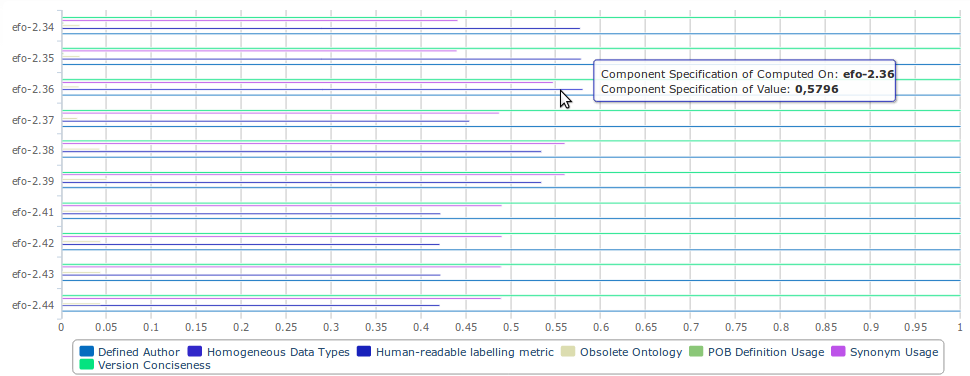
\includegraphics[scale=0.3]{images/cube_1.png}
\caption{Horizontal Bar Chart} 
  \label{fig:hor_chart}
\end{figure*}

\begin{figure*}[tbph]
\center
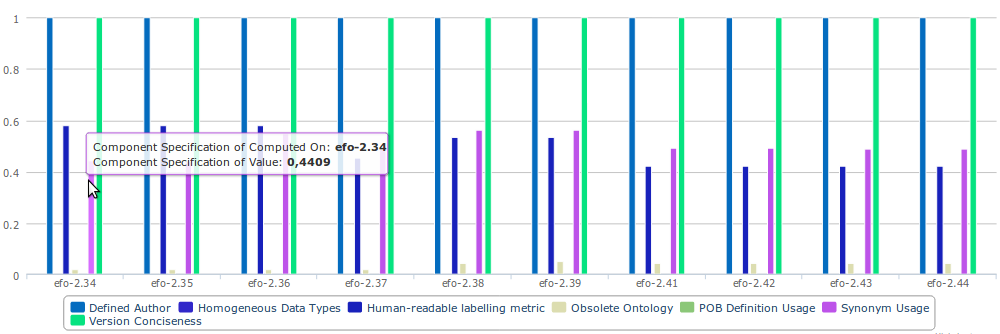
\includegraphics[scale=0.3]{images/cube_2.png} 
\caption{Vertical Bar Chart} 
\label{fig:ver_chart}
\end{figure*}

\begin{figure*}[tbph]
\center
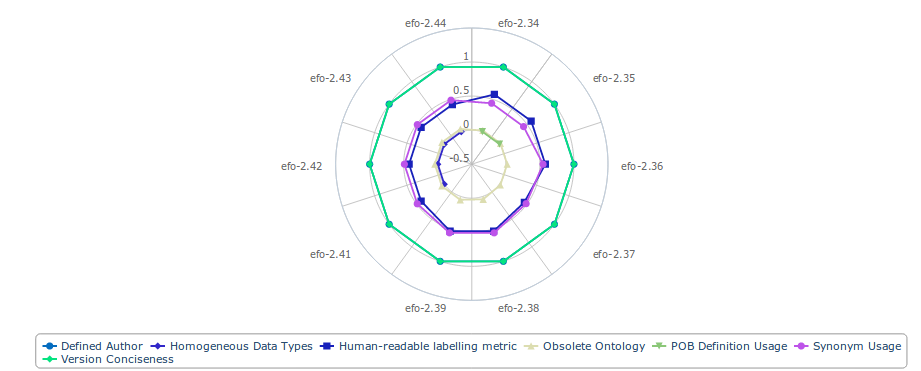
\includegraphics[scale=0.3]{images/cube_3.png} 
\caption{Radar Chart} 
\label{fig:rad_chart}
\end{figure*}

\begin{figure*}[tbph]
\center
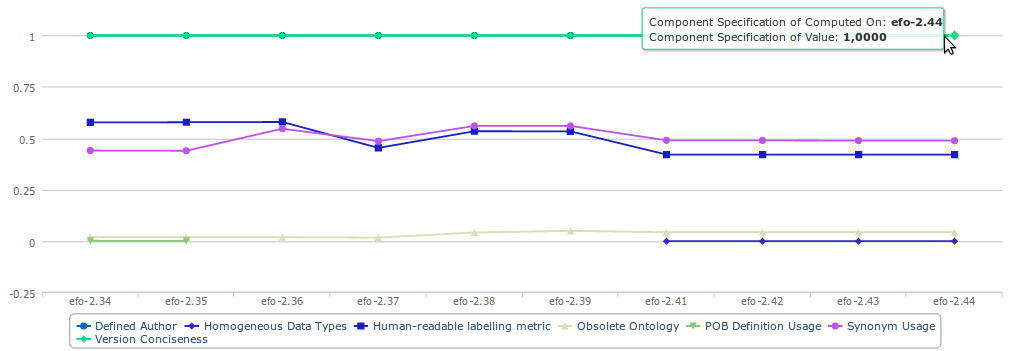
\includegraphics[scale=0.3]{images/cube_4.png} 
\caption{Lines Plot} 
\label{fig:line_chart}
\end{figure*}

A \emph{horizontal bar} represents each metric (Figure~\ref{fig:hor_chart}) and shows its value (x-axis) with respect to the dataset (y-axis).
Here, the different “datasets” analysed are actually successive revisions of one dataset.
This chart provides a clear view of how the value associated to each one of the measured metrics changes as the dataset evolves.
The horizontal layout is appropriate when the range of metric values is wide, and the number of different datasets is relatively small.

Similar to the horizontal bars chart, the \emph{vertical bar chart} (Figure~\ref{fig:ver_chart}) allows the user to compare the values computed for each of the metrics (y-axis), with respect to the dataset (x-axis).
In contrast with its horizontal counterpart, this chart is more appropriate when there are many datasets analysed but the range of metric values is not so wide.

In the \emph{radar chart} (Figure~\ref{fig:rad_chart}), the datasets are represented as slices of a circle and the values corresponding to the metrics are depicted as points and lines of a particular color.
This chart provides a clear view of how the values of the metric differ from each other for each particular dataset. 
Furthermore, it allows one to assess the overall quality of a dataset, by showing whether the values of the metrics are concentrated around sections of the circle regarded as “good” or “bad”.

The lines plot (Figure~\ref{fig:line_chart}), lists the different datasets against the values of the metrics.
Here, where “different datasets” are actually different revisions in the evolution of one dataset, this plot provides a comparison of the evolution of the quality of the dataset, with respect to each metric.
The lines emphasise the points where the values of the metrics changed noticeably from one version to the next.

% in this section we need to describe the general architecture (stream processor, daq, cache, metrics, plugins etc...) of the quality framework - including how this framework will connect to other modules in diachron